\documentclass[a4paper,twoside,master.tex]{subfiles}
\begin{document}
\lecture{13}{Wednesday, February 12, 2020}{The Legendre Transformation}

\section{Legendre Transformations}
\label{sec:legendre_transformations}

Suppose we are given a function $ f(x) $ along with its derivative $ p = p(x) = f'(x) $. Can we construct a function $ g(p) $ which contains ``the same information'' as $ f(x) $? In other words, can we construct a $ g(p) $ which can be transformed in a similar way back into $ f(x) $? Naively, we could try solving for $ x(p) $ by inverting the function $ p = f'(x) $ or $ x = f'^{-1}(p) $. Unfortunately, this is only possible if $ f' $ is monotonoic which implies $ f $ is either convex or concave. Let's assume the universe is nice and we have such a function. Now we insert $ x(p) $ into $ f(x) $ so that our new function is
\begin{equation}
    g(p) = f(x(p))
\end{equation}
This does not work, despite how nice it looks, because $ g(p) $ does not contain enough information to reconstruct $ f(x) $.
\begin{ex}
    Suppose $ f(x) = \frac{1}{2} (x-x_0)^2 $. This is a parabola, so it is convex. $ p = f'(x) = x-x_0 $ so that $ x(p) = p + x_0 $. Therefore
    \begin{equation}
        g(p) = f(x(p)) = \frac{1}{2} (p+x_0-x_0)^2 = \frac{1}{2} p^2
    \end{equation}
    We have lost all information about where the parabola is centered. The answer no longer contains $ x_0 $.
\end{ex}

We need to think about a way to specify a function via its slopes. In \Cref{fig:lec_13_convex_tangents} we see that any function can be described by its entire family of tangents. In fact, if the function is strictly convex or concave, it is bounded by its tangents and each tangent line will have a unique $ y $-intercept. We can surely use this to reconstruct the original function.


\begin{figure}[h]
    \centering
    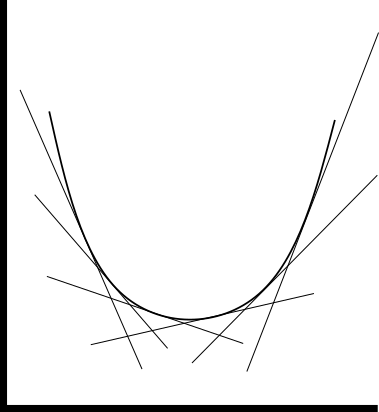
\includegraphics[width=0.5\textwidth]{figures/lec_13_function_tangents.png}
    \caption{A convex function is bounded by its tangents and each tangent has a unique $ y $-intercept}
    \label{fig:lec_13_convex_tangents}
\end{figure}

For a given point on the function, the tangent line can be described as
\begin{equation}
    t_{x_0}(x) = f(x_0) + f'(x_0) (x - x_0)
\end{equation}
The $ y $-intercept of this tangent is
\begin{equation}
    t_{x_0}(0) = f(x_0) - x_0 f'(x_0)
\end{equation}

If $ f $ is convex, then $ f'(x) $ is monotonic, and there is a unique relation between the intercept and slope. Therefore, $ p = f'(x_0) $ can be uniquely solved for $ x_0(p) $. Hence, either $ x_0 $ or $ p $ can be used to specify a given tangent. Let's use the slope to characterize the intercept:
\begin{equation}
    t_p(0) = f(x_0(p)) - x_0(p) p
\end{equation}

For any choice of $ p $, we can calculate the intercept, so we know the entire family of tangents. Therefore, for a convex or concave function, knowing the derivative gives us an exact definition of all the tangent lines.

\begin{equation}\label{eq:legendre_transform}
    g(p) = t_p(0) = f(x_0(p)) - x_0(p) p\tag{Legendre Transformation}
\end{equation}

We can formalize this as
\begin{equation}
    g(p) = \min_x\left\{ f(x) - xp \right\} \qq{convex } f
\end{equation}
For concave function, just take the maximum. Let's find the minimum:
\begin{equation}
    0 = \pdv{x}\left\{ f(x) - xp \right\} = f'(x) - p
\end{equation}
or $ p = f'(x) $. Since $ f $ is convex, we can solve this for $ x $:
\begin{equation}
    x = f'^{-1}(p) = x(p)
\end{equation}
Therefore
\begin{equation}
    g(p) = f(x(p)) - x(p) p
\end{equation}


How do we construct the reverse transformation? For any point $ x $, the point that intercepts our original line is the largest value any tangent line attains at that value of $ x $:
\begin{equation}
    \max_p\left\{ t_p(0) + px \right\} = \max_p \left\{ f(x_0(p)) - x_0(p) p + px \right\}
\end{equation}
\begin{equation}
    0 = \pdv{p}\left\{ f(x_0(p)) - x_0(p) p + px \right\} = \underbrace{\pdv{f}{x_0}}_{p} \pdv{x_0}{p} - \pdv{x_0}{p} p - x_0(p) + x
\end{equation}
so the first two terms cancel. We are left with $ x = x_0 $. Now inserting this back into our original equation, we find
\begin{equation}
    \max_p\left\{ t_p(0) + px \right\} = f(x) - xp + px = f(x):W
\end{equation}

Putting this all together, we can write this transform as a proper pair of transforms:
\begin{equation}
    g(p) = \min_x\left\{ f(x) - xp \right\}
\end{equation}
\begin{equation}
    f(x) = \max_p\left\{ g(p) + px \right\}
\end{equation}

As it turns out, there is an equivalent transformation if we swap the $ + $ and $ - $ signs in both transforms.

\begin{equation}
    g'(p) = \pdv{g}{p} = \pdv{p}\left\{ f(x(p)) - px(p) \right\} = \pdv{f}{x} \pdv{x}{p} - p \pdv{x}{p} - x(p) = - x
\end{equation}

Notice that this is the same way we defined $ p = f'(x) $ with a different sign:
\begin{equation}
    \dd{f} = p \dd{x} \qquad \dd{g} = - x \dd{p}
\end{equation}

\end{document}
